Avan\c{c}os recentes nas tecnologias de sistemas eletr\^onicos, semicondutores, sensores, microcontroladores e r\'adios tornaram poss\'ivel o desenvolvimento de redes de sensores de baixo custo e baixo consumo uma realidade.

Este cap\'itulo apresenta uma vis\~ao geral sobre redes de sensores sem fio, arquitetura orientada a servi\c{c}os e os protocolos de aplica\c{c}ao existentes.

\section{Redes de sensores sem fio}

Redes de sensores sem fio s\~ao utilizados para capturar, processar e comunicar dados captados do ambiente. Geralmente tais redes possuem centenas ou milhares de sensores e possuem as seguintes caracter\'isticas: pouca mem\'oria, pouco alcance do r\'adio, baixa capacidade de processamento e bateria, e custo reduzido.

Um n\'o pertencente a esta rede geralmente \'e um dispositivo especificamente desenvolvido para um pr\'oposito, que possui poucos recursos computacionais e energ\'eticos e se comunicam entre seus semalhantes, como apresentado na figura \ref{fig:a}.

\begin{figure}
   \label{fig:a}
   \centering
   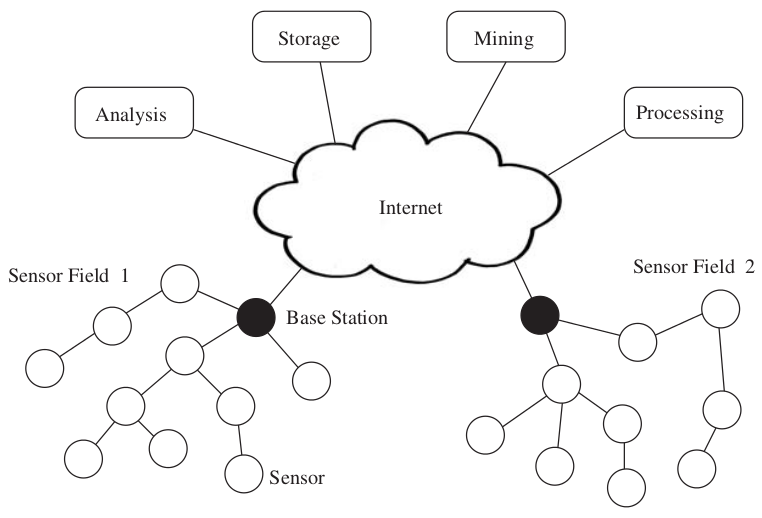
\includegraphics[width=0.7\textwidth]{figuras/wsn.png}
   \caption{Overview de uma redes de sensores sem fio}
\end{figure}

A conserva\c{c}\~ao de energia \'e um dos objetivos das redes de sensores sem fio, pois n\~ao est\~ao ligados diretamente a fonte de energia. Deve-se minimizar o consumo em todos os n\'iveis do sistema, da aplica\c{c}\~ao at\'e o meio f\'isico, iniciando com o projeto de r\'adio. \cite{WsnSurvey2008} 


\section{Arquitetura orientada a servi\c{c}os}

Arquitetura orientada a servi\c{c}os \'e uma forma de organizar infraestrutura e aplicac\c{c}\~oes de software em um conjunto de servi\c{c}os. Estes s\~ao oferecidos por prestadores de servi\c{c}o, organizac\c{c}\~oes que implementam os servi\c{c}os, fornece descri\c{c}\~ao, suporte t\'ecnico e de neg\'ocio.

Clientes destes servi\c{c}os podem ser outras solu\'c~oes, aplica\c{c}\~oes, processos ou usu\'arios.

Para satisfazer estes requis\'itos um servi\c{c}o deve:

\begin{itemize}
\item Um.
\item Dois.
\end{itemize}

\cite{perrey2003service}

\afazer{A desenvolver...}


\section{RESTful}

Um servi\c{c}o web que utiliza HTTP e os princ\'ipios REST possui recursos e a\c{c}\~oes gen\'ericas bem definidas.\cite{rest}

Para transfe\^encia de dados utiliza-se formatos gen\'ericos que enfatizam simplicidade e usabilidade pela internet, como XML e JSON.

Os Recursos s\~ao usam um identificador \'unico e persistente, as URIs. A URIs possuem estruturas de diret\'orios, uma URI \'e uma \'arvore com ramos subordinados e superordinados conectando os n\'os. As opera\c{c}\~oes suportas s\~ao m\'etodos HTTP expl\'icitos que n\~ao salvam estado das aplica\c{c}\~oes clientes e s\~ao idempotentes, s\~ao eles:
\begin{itemize}
    \item GET: solicita ao webserver a representa\c{c}\~ao de uma informa\c{c}\~ao de um determinado recurso.
    \item POST: criar um recurso no webserver.
    \item PUT: mudar o estado de um recurso do webserver.
    \item DELETE: remover o recurso ou alterar para um estado vazio.
\end{itemize}

Uma abordagem utilizando SOAP RPC em HTTP n\~ao \'e interessante para uma aplica\c{c}\~ao de RSSF, j\'a que a quantidade de informa\c{c}\~ao a ser transmitida \'e consideravelmente maior. Al\'em disso, a aplica\c{c}\~ao teria que conhecer l\'ogica interna do servi\c{c}o istrumentando o recurso utilizando chamadas de fun\c{c}\~oes remotas. A Figura 2 exemplifica e demonstra a diferen\c{c}a de uma aplica\c{c}\~ao que faz uso de SOAP RPC e outra RESTful.\cite{richardson2008restful}

%Inserir figura que demonstra a diferença entre o tamanho dos pacotes.
\afazer{A desenvolver...}

\section{CoAP}

Um dos principais objetivos do CoAP \'e ser uma alternativa protocolo web gen\'erico para redes com dispositivos com restri\c{c}\~ao de energia e mem\'oria.

As vantagens de utilizar um protocolo compat\'ivel com o HTTP s\~ao: a facilidade de integra\c{c}\~ao e o reuso de aplica\c{c}\~oes. CoAP \'e um conjunto REST otimizado para M2M, com suporte a descoberta de recursos, multicast e troca de mensagens ass\'incronas com simplicidade e baixo overhead.

A IETF estabelece as condi\c{c}\~oes m\'inimas para o desenvolvimento de um protocolo de aplica\c{c}\~ao compat\'ivel com HTTP, mas focado em aplica\c{c}\~oes aonde energia e mem\'oria s\~ao escassas. O protocolo CoAP foi projetado levando em considera\c{c}\~ao as restri\c{c}\~oes energ\'eticas e altas taxas de falha na transmiss\~ao dos pacotes em RSSF.

A comunica\c{c}\~ao entre os pontos no CoAP \'e de forma ass\'incrona usando o UDP. A confiabilidade \'e um par\^ametro opcional e funciona atrav\'es de um mecanismo de retransmiss\~ao exponencial. Possui 4 tipos de mensagem: Confirm\'avel, N\~ao-Confirm\'avel, Confirma\c{c}\~ao (ACK) e Reset. A Figura 3 mostra o formato do pacote.

\subsection{Formato das mensagens}
Uma mensagem CoAP deve caber num \'unico pacote IP, para que seja transmitida numa camada de enlace limitada.
\begin{footnotesize}
    \begin{verbatim}
    0                   1                   2                   3
0 1 2 3 4 5 6 7 8 9 0 1 2 3 4 5 6 7 8 9 0 1 2 3 4 5 6 7 8 9 0 1
+-+-+-+-+-+-+-+-+-+-+-+-+-+-+-+-+-+-+-+-+-+-+-+-+-+-+-+-+-+-+-+-+
|Ver| T |  TKL  |      Code     |          Message ID           |
+-+-+-+-+-+-+-+-+-+-+-+-+-+-+-+-+-+-+-+-+-+-+-+-+-+-+-+-+-+-+-+-+
|   Token (if any, TKL bytes) ...
+-+-+-+-+-+-+-+-+-+-+-+-+-+-+-+-+-+-+-+-+-+-+-+-+-+-+-+-+-+-+-+-+
|   Options (if any) ...
+-+-+-+-+-+-+-+-+-+-+-+-+-+-+-+-+-+-+-+-+-+-+-+-+-+-+-+-+-+-+-+-+
|1 1 1 1 1 1 1 1|    Payload (if any) ...
+-+-+-+-+-+-+-+-+-+-+-+-+-+-+-+-+-+-+-+-+-+-+-+-+-+-+-+-+-+-+-+-+
    \end{verbatim}\end{footnotesize}
\begin{center}Figura 3: formato do pacote CoAP  \cite{draft-ietf-core-coap-18}\end{center}


Os campos do pacote CoAP s\~ao:
\begin{itemize}
    \item Vers\~ao: a vers\~ao do CoAP, implementa\c{c}\~oes devem utilizar este campo com o valor 1.
    \item Tipo: campo para definir o tipo da mensagem: Confirm\'avel (0), N\~ao-Confirm\'avel (1) , de Confirma\c{c}\~ao (2) ou Reset (3).
    \item Tamanho do Token: utilizado para controle de requisi\c{c}\~oes e repostas. O tamanho do Token pode variar entre 0 e 8 bytes. Tamanhos entre 9 a 15 s\~ao reservados e n\~ao devem ser usados. \'E um campo sempre gerado pelo cliente CoAP.
    \item C\'odigo: separados em 3-bit mais significativos para classes e 5-bits menos significativos para detalhe. As classes podem indicar uma requisi\c{c}\~ao (0), uma resposta de sucesso (2), e uma resposta de erro do cliente (4), ou uma resposta de erro do servidor (5), as outras classes s\~ao reservadas. Em um caso especial o c\'odigo 0.00 indica uma mensagem vazia.
    \item ID da mensagem: usada para deduplica\c{c}\~ao de mensagens e confirma\c{c}\~ao ou reset de mensagens.
\end{itemize}

O ID da mensagem \'e gerado por quem envia a mensagem, no caso de uma mensagem confirm\'avel ou reset, a resposta deve possuir o ID da mensagem enviada. A implemeta\c{c}\~ao da gera\c{c}\~ao dos IDs est\'a aberta, depende da aplica\c{c}\~ao que o CoAP ser\'a usado, por\'em \'e recomendado que o valor inicial seja rand\^omico.
   
%Codifica\c{c}\~ao das op\c{c}\~oes
\subsection{Transmiss\~ao de Mensagens}
A transmiss\~ao de mensagems \'e controlada basicamente pelos par\^ametros:

\begin{itemize}
    \item ACK TIMEOUT: tempo que uma mensagem confirm\'avel aguarda o ACK.
    \item ACK RANDOM FACTOR: fator de randomicidade para gerar os ACK TIMEOUTs subsequentes.
    \item MAX RETRANSMIT: contador para o n\'umero m\'aximo de tentativas de retransmiss\~ao.
    \item NSTART: n\'umero limite de intera\c{c}\~oes simult\^aneas mantidas por um servidor.
    \item Leisure: tempo que o servidor aguarda para responder uma requisi\c{c}\~ao multicast, \'e calculada: \begin{math}Leisure = S * G / R\end{math}. Aonde S \'e o tamanho estimado da reposta, G \'e uma estimativa do tamanho do grupo e R \'e a taxa de transmiss\~ao.
    \item PROBING RATE: \'e a taxa m\'edia para transmiss\~ao de dados.
\end{itemize}

Estes par\^ametros definem a temporiza\c{c}\~ao do sistema. Os valores padr\~oes s\~ao mostrados na Tabela 1.
\begin{center}
\begin{verbatim}
            +-------------------+---------------+
            | name              | default value |
            +-------------------+---------------+
            | ACK_TIMEOUT       | 2 seconds     |
            | ACK_RANDOM_FACTOR | 1.5           |
            | MAX_RETRANSMIT    | 4             |
            | NSTART            | 1             |
            | DEFAULT_LEISURE   | 5 seconds     |
            | PROBING_RATE      | 1 Byte/second |
            +-------------------+---------------+
\end{verbatim}
Tabela 1
\end{center}

A retransmiss\~ao \'e controlada por um timeout e um contador. Quando este timeout \'e atigido e o contador \'e menor que valor m\'aximo de retransmiss\~ao a mensagem \'e transmitida, o contador incrementado e timeout duplicado.

Uma falha na transmiss\~ao ocorre quando atingir o n\'umero m\'aximo de tentavivas ou receber uma mensagem de RESET. Quando receber um ACK a transmiss\~ao da mensagem confirm\'avel \'e completa.

O servidor ir\'a ignorar mensagens que chegam por multicast quando n\~ao puder responder nada de \'util.
Na situa\c{c}\~ao aonde possuir uma informa\c{c}\~ao suficientemente nova pode responder na pr\'opria mensagem de confirma\c{c}\~ao (ACK). Essa t\'ecnica \'e chamada de ''Piggy-backed'' um mecanismo de transmiss\~ao para mensagens confirmadas, o cen\'ario \'e ilustrado na Figura 4.\cite{draft-ietf-core-coap-18}

\begin{center}
\begin{verbatim}
Client  Server
    |      |
    |      |
    +----->|     Header: GET
    |      |  (T=CON, Code=0.01, MID=0x7d34)
    | GET  |   Uri-Path: "temperature"
    |      |
    |<-----+     Header: 2.05 Content
    |      |  (T=ACK, Code=2.05, MID=0x7d34)
    | 2.05 |    Payload: "22.3 C"
    |      |
\end{verbatim}
Figura 4
\end{center}

\subsection{Camada de Reposta e Requisi\c{c}\~ao}
Uma requisi\c{c}\~ao \'e inicializada ao preencher o campo code no cabe\c{c}alho do CoAP. Possuem as mesmas propriedades de idempot\'encia e only retrieved das requisi\c{c}\~oes HTTP.


O modelo de requisi\c{c}\~ao e resposta usa um contador de timeouts. E a retransmiss\~ao das mensagens \'e defina por uma fun\c{c}\~ao que varia de acordo com o n\'umero de tentativas.
 

\subsection{Recursos}
A descoberta de recursos \'e feita quando um servidor recebe uma requisi\c{c}\~ao GET para o recurso ~/well-know/core. O servidor CoAP deve responder no formato CORE link Format.\cite{rfc6690} E a descoberta de servi\c{c}os no protocolo CoAP \'e feita atrav\'es de socket Multicast. Os recursos s\~ao identificados por uma URI, e os m\'etodos s\~ao implementados de forma similar ao HTTP.

\afazer{A desenvolver...}

%Inserir figura que represente os recursos ???

\section{EPOS}
O EPOS \'e um sistema operacional multithread com suporte a preemp\c{c}\~ao, foi desenvolvido em C++ que faz uso intenso de programa\c{c}\~ao orientada a aspectos utilizando templates.

Possui abstra\c{c}\~oes para entidades temporais como rel\'ogio, alarme e cron\^ometro, biblioteca com estruturas de dados e sequenciadores. Permitindo o uso de ferramentas para gera\c{c}\~ao automatizada de abstra\c{c}\~oes de sistemas. A portabilidade \'e atingida utilizando entidades chamados de Mediadores de Hardware que fornecem interfaces simples para acesso as fun\c{c}\~oes espec\'ificas de arquitetura. Estas interfaces s\~ao utilizadas por entidades abstratas como alarmes e threads peri\'odicas. A figura 5 mostra uma vis\~ao abstrata da arquitetura do EPOS.

%Inserir figura da arquitetura do EPOS.

Foi projetado utilizando ADESD, Application Driven Embedded System Design, um m\'etodo para projeto de sistemas embarcados orientados \`a aplica\c{c}\~ao. Esta metodologia guia o desenvolvimento paralelo de hardware e software al\'em de manter portabilidade. O EPOS possui porte para as seguintes arquiteturas: MIPS, IA32, PowerPC, H8, Sparc, AVR e ARM. \cite{epos}

Utiliza um sistema de constru\c{c}\~ao baseado em makefiles e shell scripts.

\section{Trabalhos Relacionados}

\subsection{Contiki}
O Contiki \'e um sistema operacional criado por Adam Dunkels em 2000, escrito em C, de c\'odigo aberto para sistemas com restri\c{c}\~ao de recursos comunicam-se numa rede. Foi desenvolvido para ser um sistema operacional para Internet das coisas. Possui uma camada de abstra\c{c}\~ao RESTful para web services chamada Erbium, que implementa o protocolo CoAP.

Cada processo no Contiki possui bloco de controle, que cont\'em informa\-\c{c}\~oes de tempo de execu\c{c}\~ao do processo e uma refer\^encia para uma protothread, na qual o c\'ogido \'e armazenado na ROM. 

Protothread \'e uma combina\c{c}\~ao entre eventos e threads, possuem comportamentos de bloqueio e espera, que permite o intersequenciamento dos eventos, gerando um baixo overhead de mem\'oria por n\~ao necessitar de salvamento de contexto.

Cada protothread consome 2 bytes de mem\'oria, que s\~ao utilizados para armazenar a continuidade local, uma referencia utilizada em um pulo condicional durante a execu\c{c}\~ao da thread. \'E um m\'etodo similar ao mecanismo de Duffy e Co-rotina em C. \cite{duffy}

O transceiver sem fio \'e um dos componentes que mais consome energia quando ligado escutando o ambiente, assim uma das estrat\'egias utilizadas \'e manter o m\'inimo de tempo poss\'ivel ligado, mas o suficiente para manter a troca de mensagens na rede. O Contiki prop\~oe uma estrat\'egia de ciclos de trabalho que consegue manter um n\'o comunic\'avel em uma rede, por\'em com seus r\'adios desligados em aproximadamente 99\% do tempo.

\subsection{LibCoap}
LibCoap \'e uma biblioteca implementada em C do protocolo CoAP. Possui 292K de tamanho compilada estaticamente em sua vers\~ao 4.0.1.


\subsection{TinyOS}
O TinyOS \'e um sistema operacional projetado para sistemas embarcados com comunica\c{c}\~ao sem fio e restri\c{c}\~oes energ\'eticas. Foi desenvolvido em nesC, uma linguagem c\'odigo aberto que \'e uma extens\~ao do C. \'E um sistema operacional baseado em eventos desenvolvido para redes de sensores que possuem recursos limitados. Possui uma implementa\c{c}\~ao do CoAP baseada na libCoAP.
